
\paragraph{Experiments preparation and data collection}

% Cenni al experiment_handler
The set of experiments and data collected in the laboratory requires a systemathic way to organize and manage them. Hence, Matlab functions have been designed: they help us in defining new experiments, which control techinque using, which data types recording and analysing.

\section{Available sensors} \label{sec:sensors}

The setup includes three sensors: a potentiometer on the motor shaft and an encoder for each mass.

\paragraph{Potentiometer}

The potentiometer is installed next to the gear, on the load side. It is a single turn~$10 \ k\Omega$ sensor with no physical stops and has an electrical range of 352°; by definition, this sensor provides an absolute position measurement. \\
\begin{figure*}[h]
	\centering
	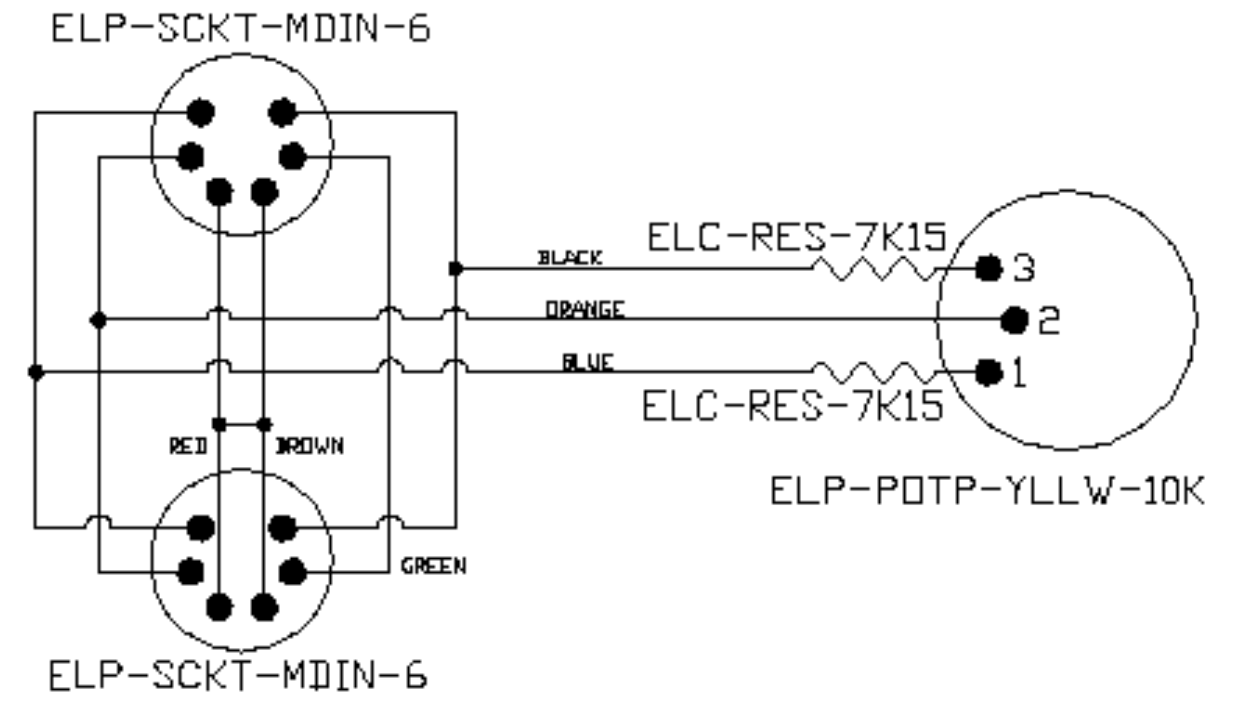
\includegraphics[width=0.4\columnwidth]{potentiometer_scheme}
	\caption{Potentiometer electrical scheme}
\end{figure*}
% trasformazione volt->rad fallita: non viene letta +-5V ma di meno
% tolto il modulo, per avere posizione incrementale su più giri
% interpolazione dei punti mancanti negli 8° di buco
% osservazione che pendenza della posizione è scorretta (causa tensione imprecisa)
% impossibilità di usare potenziometro come sensore di posizione/velocità durante il funzionamento, ma solo come posizione iniziale
% potenziomentro comunque impreciso di per sé

The total output range of the sensor should be ±5 V over the full 352° range.
Ideally, the first passage to obtain the motor position is converting the voltage measured in radiant:
\[
	\theta_l = \bigl{(} V_{meas} - V_1 \bigr{)} \frac{352 \degree }{V_3 - V_1} \frac{\pi}{180 \degree }
\]

\subparagraph{Sensor calibration}
Actually, a variation of the voltage range must be considered: at the ends of the potentiometer sensor, voltage reading is not exactely $\pm 5V$, due to resistance variations from the nominal value. By observing the data collected, the usual maximum and minimum voltages are respectively~$V_3=4.67 \ V$ and~$V_1=-4.88 \ V$.

The sensor is able to detect the position along only one turn, then an incremental position that considers also the number of turns must be computed via software.
In particular, a MATLAB script for post-processing elaboration of data has been written. This is able to recognize the end of a turn and the beginning of the next one; thanks to this, it remembers the number of revolutions and rearranges all the data according to that.

Moreover, the gap of~$8 \degree$ can be fitted by interpolating the two values around it. Notice that this procedure works only in case the motor speed is quite constant in time.
\begin{figure*}[h]
	\centering
	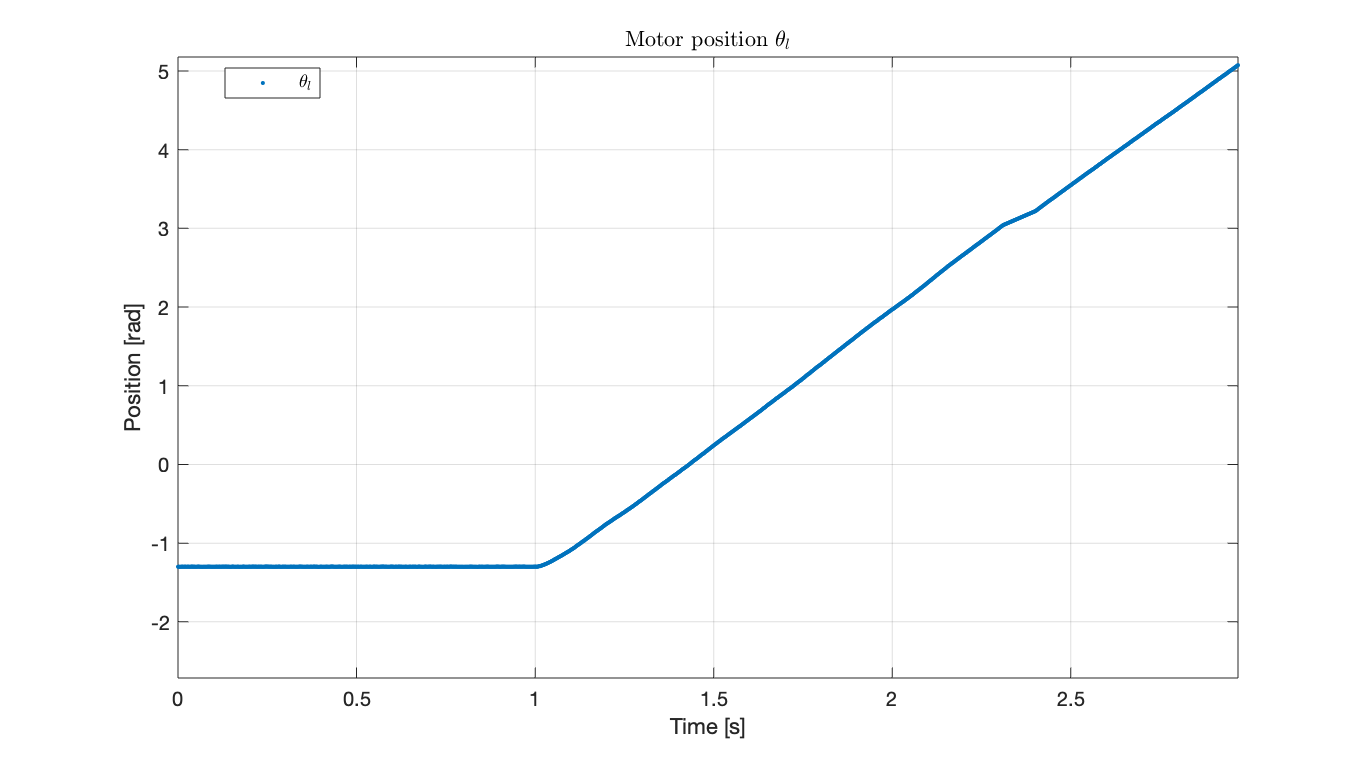
\includegraphics[width=\columnwidth]{pote_recover}
	\caption{Potentiometer data post-processing}
\end{figure*}
% figure script potentiometer

Unfortunately it is visible that the sensor data are quite imprecise: the slope of the curve is not continuous. For this reason, real time measurements for motor position and speed are reliable only in its range of functioning.
\begin{itemize}
	\item gray-box model identification (after post-processing);
	\item initial condition for absolute position control;
	\item motor position measurement, for control in state-space form (range of reference is~$-\frac{352 \degree}{2} \, / +\frac{352 \degree}{2}$).
\end{itemize}

\subparagraph{Uncertainty and noise}
Even when the system is steady, we can see that the motor position measurement oscillates; this is due to an error in voltage measurement performed by the ADC. It is treated as a white-noise, whose variance is determined in Matlab, using data collected in steady condition.

\begin{align*}
	\Theta_{pot} &\sim \Gamma \bigl{(} 0, 1e-6 \bigr{)}
\end{align*}

\paragraph{Encoder}

The encoder is a digital sensor that reads angular motions. It generates a pulse every small movement (both clockwise or counter-clockwise, detecting the direction of the motion) and, thanks to a counter, gives an incremental measurement with respect to the initial position. One revolution includes 4096 pulses, so the formula to obtain the position is the following:
\[
	\theta_x = \frac{2\pi}{4096} \ y \qquad x={1,2}
\]
The~$y$ signal is the processed one by the following Matlab function:
\begin{verbatim}
	function y = fcn(u)
	persistent oldu;
	persistent buffer;
	persistent oldy;
	if isempty(oldu)
		oldu=0;
		oldy = 0;
		buffer = 0;
	end
	
	% subtract the very first value of the experiment
	if u~=0 & oldu==0 
		oldu=u;
	end
	y=u-oldu;
	
	% count buffer overflows
	if ( y - oldy > 33000 )
		buffer = buffer-1;
	elseif ( y - oldy < - 33000 )
		buffer = buffer+1;
	end
	oldy = y;
	
	% add the pulses lost to overflow 
	y = y + buffer*2^16;
\end{verbatim}
This code is able to impose the initial condition of the masses position to 0 (is to be noted that the buffer is not reset after an experiment, hence it will result in an incorrect value at the beginning of the motion of the following experiment). Moreover, it must be considered that the buffer storage has dimention 16 bits, with values between $-32.768$ and $32.767$. Once a limit of the buffer is reached, an overflow occurs and the MATLAB function is able to overcome this problem by returning a greater number. The result is the correct relative motion from the beginning of the experiment.

\subparagraph{Uncertainty and noise}

The digital encoder has a resolution determined by the number of pulses per revolution:
\[
	R = \frac{1}{4096}
\]
Thus, each measurement can be seen as a uniform distribution of probability between the two adjacent pulses; the distance of the true position from the measured one can be expressed as a Gaussian probability distribution function, whose variance defines the measurement uncertainty:
\begin{align*}
	U &= \frac{(2R)^2}{12} \\
	\Theta_{enc} &\sim \Gamma \bigl{(} 0,\frac{(2R)^2}{12} \bigr{)} = \Gamma \bigl{(} 0, 2e-8 \bigr{)}
\end{align*}

\subparagraph{Speed}

The speed of the two masses is obtainable by derivating the measument of the encoders. It is done thanks to the \textit{Discrete Derivative} Simulink block, that differentiates two consecutive values with respect to the sampling time:
\[
	\dot{\theta_1} = \frac{ \theta_{enc}(t) - \theta_{enc}(t-1)}{T_s}
\]
Due to the uncertainty of the encoder, the speed derivation is noisy, according to the following:
\begin{align*}
	U &= \frac{2(2R)^2}{12 {T_s}^2 } \\
	\dot{\Theta}_{enc}	&\sim \Gamma \bigl{(} 0,\frac{(2R)^2}{12 \ {T_s}^2} \bigr{)} + \Gamma \bigl{(} 0,\frac{(2R)^2}{12 \ {T_s}^2} \bigr{)} = \Gamma \bigl{(} 0, 0.001 \bigr{)}
\end{align*}
The uncertainty of the speed is extremely higher that the position one, so a low-pass filter is needed in order to reduce the measurement noise. The cutting frequency of the filter is determined by the higher resonance frequency of the system (shown later), such that the measurement is accurate up to that value:
\[
	F_{lp} = \frac{ \omega_f }{ s+\omega_f} \qquad \omega_f=25Hz=157.08 rad/s
\]